\section{Recolección de datos y definición del modelo}

Para la construcción del modelo se realizó un relevamiento del funcionamiento
de la guardia pediátrica del Hospital Vilela, considerando tanto su
distribución física como los recursos y procesos involucrados.

La información fue obtenida principalmente a partir del conocimiento aportado
por una residente del hospital y complementada con estimaciones realizadas
por el grupo cuando no se contó con registros históricos específicos. En
estos casos los valores se consideran supuestos del modelo y se contrastan
durante la etapa de validación.

\subsection{Representación física del sistema}

El modelo se construyó sobre un plano de la guardia que representa las
principales áreas involucradas en el recorrido del paciente: acceso principal,
acceso de ambulancias, secretaría, sala de espera, consultorio de triage,
cuatro consultorios médicos, Shock Room y sector de internación.

\begin{figure}[H]
  \centering
  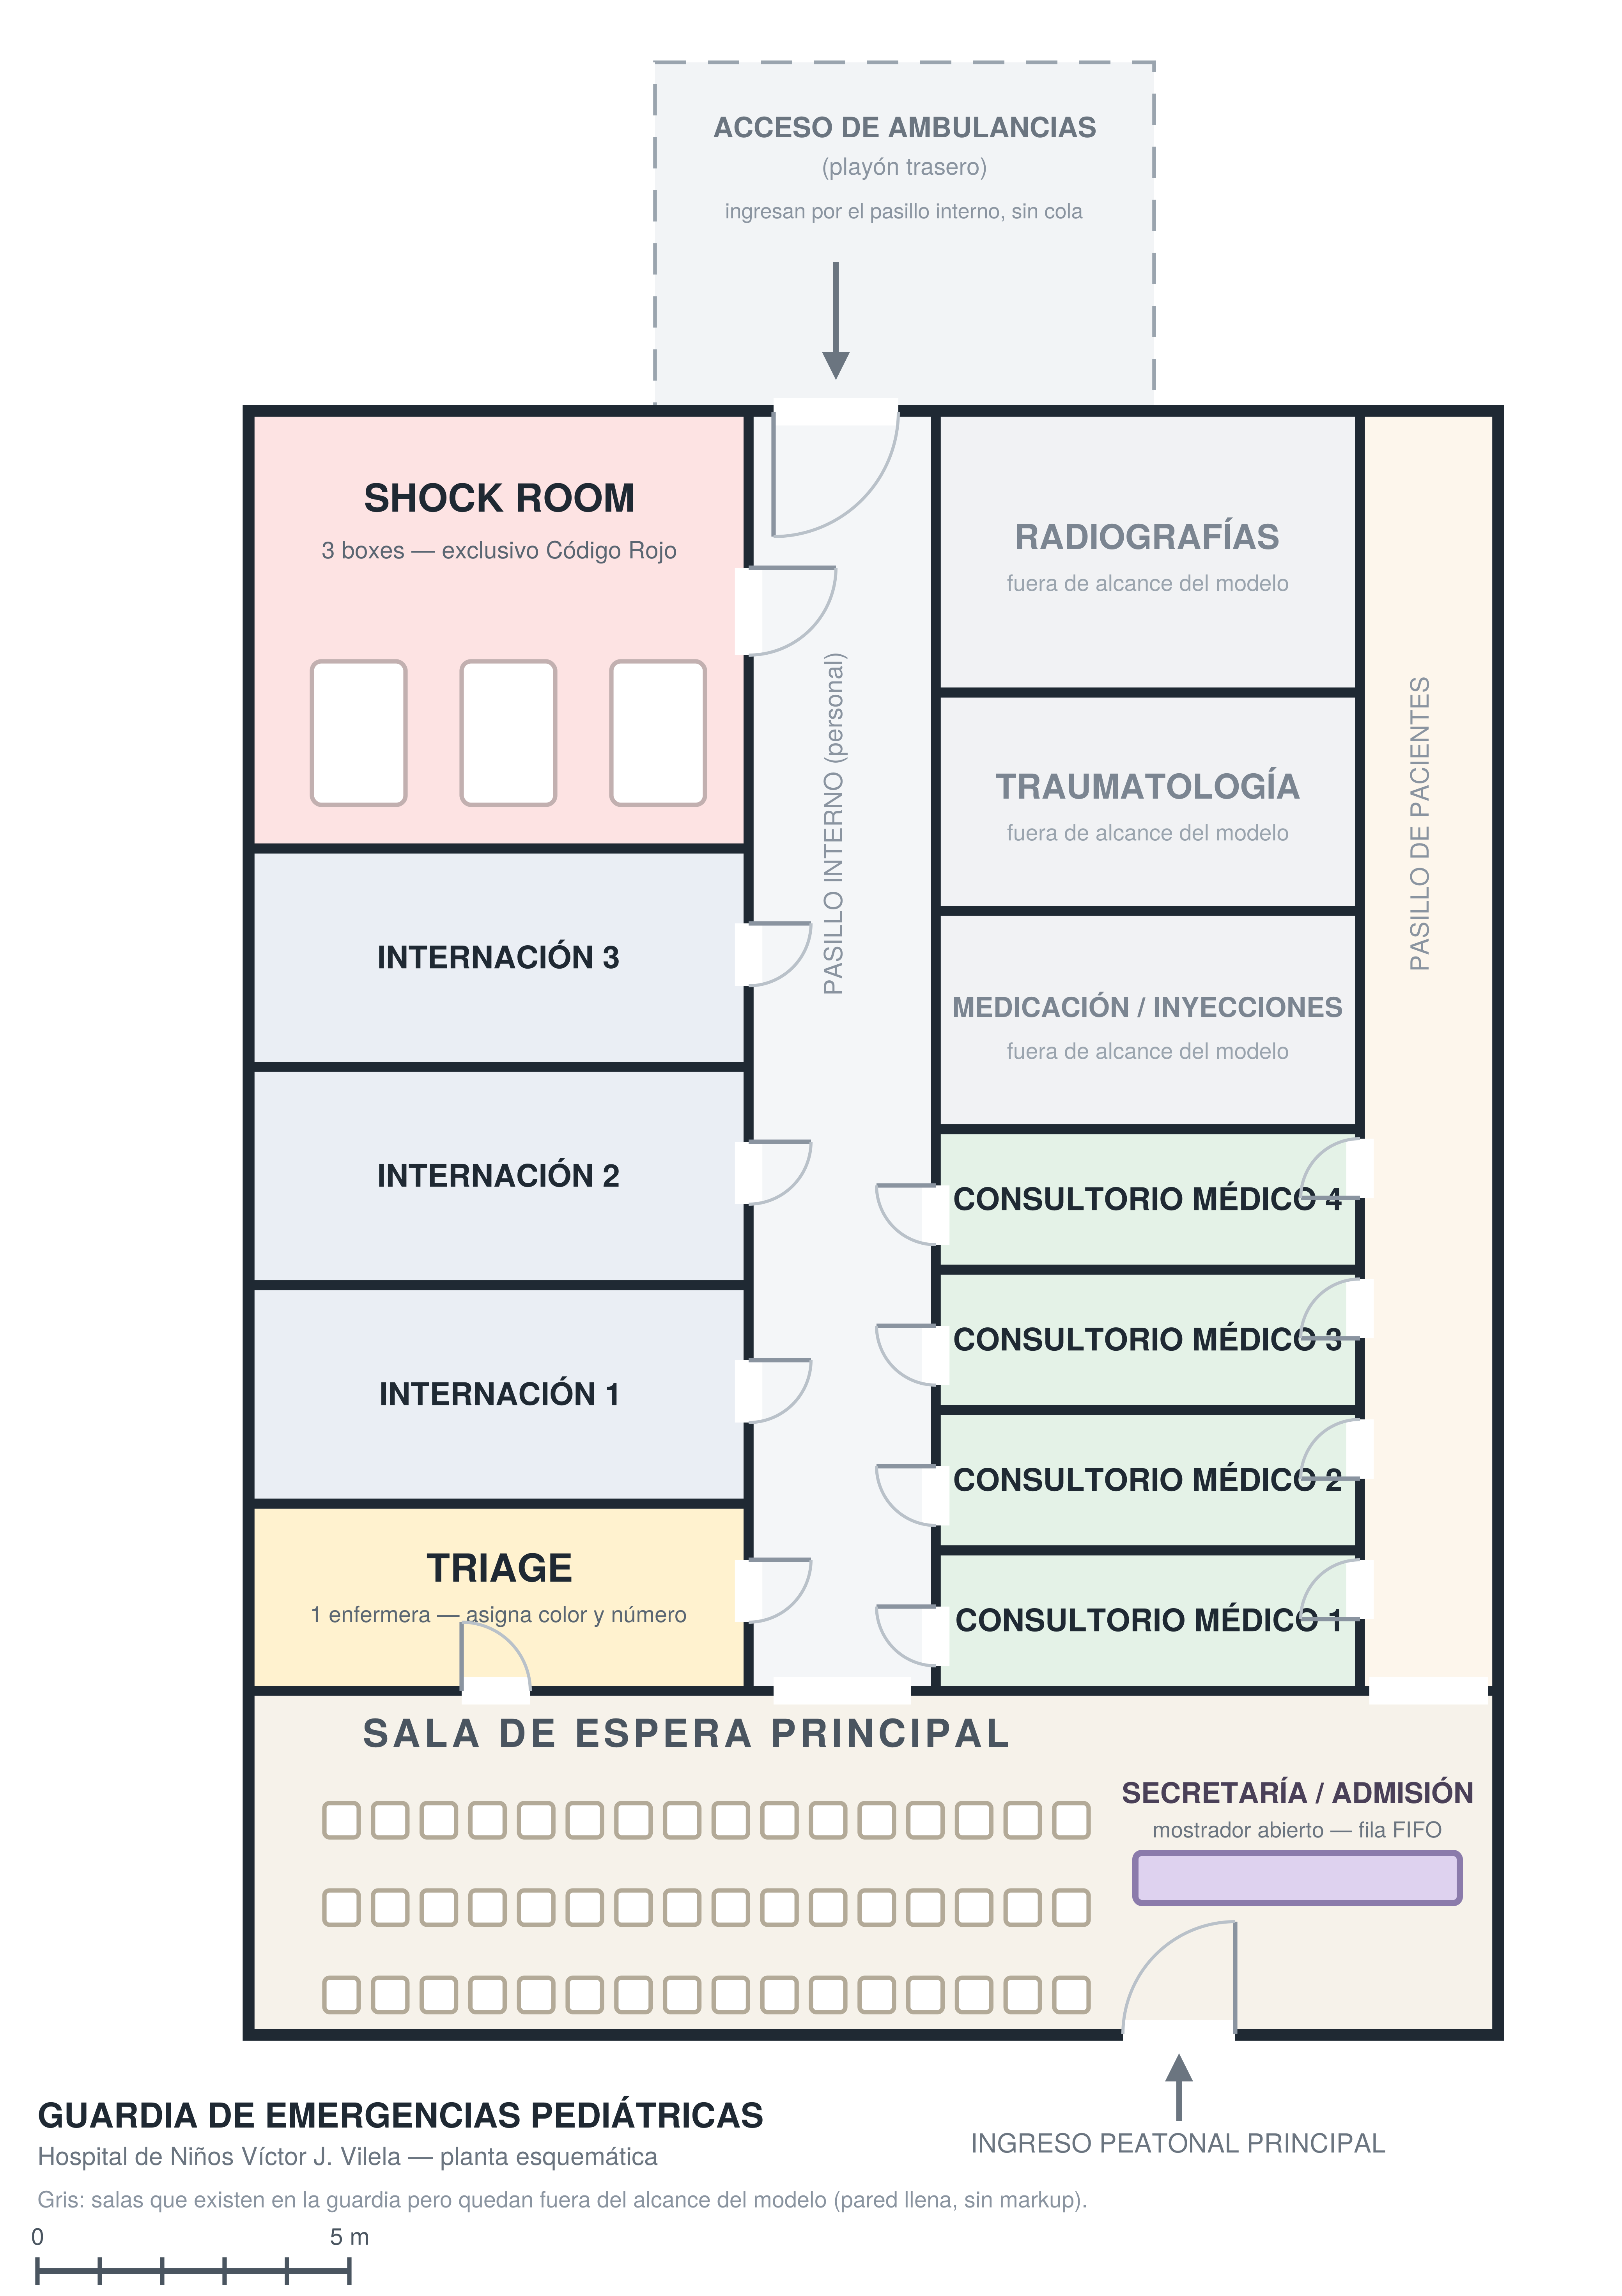
\includegraphics[width=0.85\textwidth]{plano_guardia_vilela.png}
  \caption{Plano de la guardia utilizado como base del modelo. Los sectores
  de traumatología, radiografías y medicación se representan en gris por
  encontrarse fuera del alcance.}
  \label{fig:plano}
\end{figure}

El plano permite representar tanto el recorrido físico de los pacientes como
la ubicación de los distintos puntos de atención, y es el soporte sobre el
cual la Pedestrian Library de AnyLogic calcula los desplazamientos.

\subsection{Entidad y atributos del modelo}
\label{sec:entidad}

La entidad principal es el paciente pediátrico. Cada paciente lleva consigo
los atributos que determinan su comportamiento dentro del sistema:

\begin{table}[H]
\centering
\begin{tabular}{lll}
\toprule
\textbf{Atributo} & \textbf{Tipo} & \textbf{Significado} \\
\midrule
\texttt{colorReal}            & \texttt{ColorTriage} & Gravedad clínica real \\
\texttt{codigo}               & \texttt{ColorTriage} & Color asignado en el triage \\
\texttt{prioridad}            & \texttt{int}         & Prioridad en la cola, derivada de \texttt{codigo} \\
\texttt{porAmbulancia}        & \texttt{boolean}     & Forma de ingreso \\
\texttt{detectadoEnPuerta}    & \texttt{boolean}     & Rojo identificado en el acceso \\
\texttt{destino}              & \texttt{Destino}     & Alta o internación \\
\texttt{consultorioAsignado}  & \texttt{int}         & Consultorio en que fue atendido \\
\texttt{tLlegada}             & \texttt{double}      & Instante de arribo \\
\texttt{tEntraColaTriage}     & \texttt{double}      & Ingreso a la cola de triage \\
\texttt{tInicioTriage}        & \texttt{double}      & Comienzo de la clasificación \\
\texttt{tFinTriage}           & \texttt{double}      & Fin de la clasificación \\
\texttt{tEntraColaConsultorio}& \texttt{double}      & Ingreso a la cola de prioridad \\
\texttt{tInicioConsulta}      & \texttt{double}      & Comienzo de la atención médica \\
\texttt{tSalida}              & \texttt{double}      & Egreso del sistema \\
\texttt{cuentaParaMetrica}    & \texttt{boolean}     & Pertenencia a la ventana de medición \\
\bottomrule
\end{tabular}
\caption{Atributos del agente \texttt{Paciente}.}
\end{table}

La distinción entre \texttt{colorReal} y \texttt{codigo} es central en este
trabajo y se desarrolla en la sección~\ref{sec:error}.

\subsection{Recursos y servidores}

A partir del relevamiento se consideran los siguientes recursos:

\begin{table}[H]
\centering
\begin{tabular}{llc}
\toprule
\textbf{Recurso} & \textbf{Disciplina de la cola} & \textbf{Servidores} \\
\midrule
Secretaría / admisión   & FIFO                    & 2 \\
Triage                  & FIFO                    & 1 \\
Consultorios médicos    & Prioridad no expulsiva  & 4 \\
Shock Room              & FIFO                    & 3 equipos, 8 camas \\
\bottomrule
\end{tabular}
\caption{Configuración base de recursos.}
\label{tab:recursos}
\end{table}

En el Shock Room se distingue el espacio físico de la capacidad de atención:
el sector dispone de ocho camas, pero sólo tres pacientes pueden ser
atendidos simultáneamente por limitación de personal. Esta distinción se
implementa mediante una cola de capacidad ocho y un conjunto de recursos de
capacidad tres.

\subsection{Flujo de pacientes}

El paciente peatonal atraviesa las siguientes etapas:

\begin{center}
Ingreso $\rightarrow$ Secretaría $\rightarrow$ Sala de espera $\rightarrow$
Triage $\rightarrow$ Sala de espera $\rightarrow$ Consultorio $\rightarrow$
Alta / Internación
\end{center}

Corresponde notar que el paciente atraviesa la sala de espera dos veces: una
vez antes del triage, en cola FIFO, y otra después, en cola ordenada por
prioridad. Ambas colas comparten el mismo espacio físico, lo que resulta
relevante para la métrica de hacinamiento.

Una fracción de los pacientes peatonales presenta un cuadro crítico
identificable en el acceso. Estos casos se derivan directamente al Shock Room
sin pasar por secretaría ni triage, igual que los pacientes de ambulancia.

\subsection{Clasificación y prioridad de atención}

Durante el triage los pacientes se clasifican en cuatro categorías. La
distribución estimada para un día pico invernal y las prioridades asociadas
son:

\begin{table}[H]
\centering
\begin{tabular}{lcc}
\toprule
\textbf{Código} & \textbf{Proporción} & \textbf{Prioridad} \\
\midrule
Rojo     & 1,0 \%  & 4 \\
Naranja  & 7,2 \%  & 3 \\
Amarillo & 25,5 \% & 2 \\
Verde    & 66,3 \% & 1 \\
\bottomrule
\end{tabular}
\caption{Distribución de gravedad real y prioridad de atención.}
\label{tab:colores}
\end{table}

\begin{pendiente}
El documento de avance anterior consignaba una proporción de pacientes rojos
del 3~\%, mientras que el modelo implementa 1~\%. Debe unificarse el valor y
dejar constancia del criterio adoptado.
\end{pendiente}

\subsection{Proceso de llegada}
\label{sec:arribos}

El Hospital Vilela registra aproximadamente 97.000 consultas anuales por
guardia, lo que equivale a unos 266 pacientes diarios. Distribuidos de manera
uniforme a lo largo de las 24 horas representarían alrededor de 11 pacientes
por hora.

El modelo implementado utiliza una tasa constante de \textbf{10 pacientes por
hora} para el ingreso peatonal y \textbf{0,2 por hora} para el ingreso en
ambulancia, sobre una ventana de ocho horas correspondiente al turno
vespertino. Este valor fue consultado con una profesional que se desempeña en
la guardia, quien lo consideró razonable para el día modelado.

Los arribos se modelan mediante un proceso de Poisson, que constituye el
supuesto estándar para llegadas independientes a un servicio de urgencias.

\begin{pendiente}
El documento de avance anterior proponía una tasa \emph{variable por franja
horaria} (13, 16, 18, 20, 19 y 16 pacientes por hora entre las 14:00 y las
20:00, aproximadamente 102 pacientes en seis horas), mientras que el modelo
implementa una tasa constante de 10 por hora durante ocho horas,
aproximadamente 80 pacientes. Las dos definiciones son incompatibles y debe
elegirse una. Debe tenerse presente que con la capacidad actualmente
representada en el modelo, una tasa media de 17 pacientes por hora conduce a
una utilización de los consultorios superior a la unidad, es decir, a un
sistema que no alcanza régimen estacionario.
\end{pendiente}

\subsection{Tiempos de servicio}

Los tiempos de atención se modelan mediante distribuciones triangulares. Esta
elección responde a una indicación de la cátedra y a una razón metodológica:
la triangular se define con tres valores --- mínimo, moda y máximo --- que es
precisamente lo que una persona con experiencia en el servicio puede estimar
en ausencia de registros históricos, y además no produce valores negativos.

\begin{table}[H]
\centering
\begin{tabular}{lc}
\toprule
\textbf{Proceso} & \textbf{Distribución (minutos)} \\
\midrule
Secretaría                  & triangular(1,5;\ 2,5;\ 4) \\
Triage                      & triangular(3;\ 5;\ 8) \\
Consulta verde              & triangular(10;\ 15;\ 22) \\
Consulta amarilla           & triangular(18;\ 25;\ 35) \\
Consulta naranja y roja     & triangular(35;\ 42;\ 50) \\
Atención en Shock Room      & triangular(60;\ 90;\ 150) \\
\bottomrule
\end{tabular}
\caption{Distribuciones de los tiempos de servicio.}
\label{tab:tiempos}
\end{table}

Los valores modales son consistentes con el relevamiento previo. Los extremos
de las distribuciones se consideran supuestos del grupo y deben revisarse
durante la validación.

\subsection{Destinos finales}

Una vez finalizada la atención el modelo considera dos destinos posibles:

\begin{table}[H]
\centering
\begin{tabular}{lcc}
\toprule
\textbf{Código real} & \textbf{Internación} & \textbf{Alta} \\
\midrule
Rojo     & 100 \% & 0 \% \\
Naranja  & 60 \%  & 40 \% \\
Amarillo & 20 \%  & 80 \% \\
Verde    & 2 \%   & 98 \% \\
\bottomrule
\end{tabular}
\caption{Probabilidad de internación según gravedad real.}
\label{tab:destinos}
\end{table}

Para el código rojo la derivación a internación no se modela como una
probabilidad sino como una regla del servicio: todo paciente cuya gravedad
real es roja termina internado.

Es importante señalar que el destino depende de \texttt{colorReal} y no de
\texttt{codigo}. Un paciente mal clasificado espera más o menos de lo que le
corresponde, pero su cuadro clínico --- y por lo tanto su destino --- no se
modifica por el error de clasificación.

\begin{pendiente}
La probabilidad de internación del código naranja permanece abierta entre
60~\% y 85~\%. El modelo implementa 60~\%.
\end{pendiente}

\subsection{Modelado explícito del error de triage}
\label{sec:error}

El modelo distingue la gravedad clínica real del paciente del color que le
asigna la enfermera. Esa diferencia es exactamente el sobre-triage y el
sub-triage, y constituye el objeto central del estudio.

\begin{itemize}
  \item \texttt{colorReal} se sortea al momento del arribo según la
  distribución de la tabla~\ref{tab:colores}. Determina cuánto dura la
  consulta y si el paciente termina internado.
  \item \texttt{codigo} se obtiene al finalizar el triage aplicando una
  función de clasificación sobre \texttt{colorReal}. Determina la prioridad
  en la cola de acceso al consultorio.
\end{itemize}

Cuando ambos coinciden, la clasificación fue correcta. Cuando no, el paciente
espera un tiempo que no corresponde a su gravedad.

La función de clasificación desplaza el color un escalón en la escala de
urgencia con probabilidad $p_{sub}$ hacia abajo y $p_{sobre}$ hacia arriba:

\begin{lstlisting}
double u = uniform();
if (u < pSubtriage) {
    switch (real) {
        case ROJO:     return ColorTriage.NARANJA;
        case NARANJA:  return ColorTriage.AMARILLO;
        default:       return ColorTriage.VERDE;
    }
}
if (u < pSubtriage + pSobretriage) {
    switch (real) {
        case VERDE:    return ColorTriage.AMARILLO;
        case AMARILLO: return ColorTriage.NARANJA;
        default:       return ColorTriage.ROJO;
    }
}
return real;
\end{lstlisting}

Los valores adoptados son $p_{sub} = 0{,}12$ y $p_{sobre} = 0{,}08$.

Debe notarse que la tasa de error \emph{observada} resulta menor que la
nominal, porque los extremos de la escala no pueden desplazarse más allá de
sí mismos: un paciente verde no puede ser sub-triado ni un rojo
sobre-triado. Dado que el verde representa cerca de dos tercios de los
arribos, la proporción efectiva de sub-triage se ubica en torno al 4~\%.

\begin{pendiente}
Los valores de $p_{sub}$ y $p_{sobre}$ son estimaciones del grupo sin
respaldo documental. Deben declararse como supuestos o sustituirse por
valores relevados.
\end{pendiente}

\subsection{Variables de entrada y de salida}

Las principales variables de entrada son la tasa de llegada, la distribución
de pacientes por código, la cantidad de servidores de cada tipo, los tiempos
de servicio, las probabilidades de internación y las tasas de error de
clasificación.

Como variables de salida se registran el tiempo de espera para el triage, el
tiempo de espera para el consultorio --- global y segregado por código ---,
el tiempo total de permanencia, la cantidad promedio de pacientes en la sala
de espera, la utilización de los recursos y los recuentos de sub y
sobre-triage.

